\documentclass[12pt]{article}
\usepackage[utf8]{inputenc}
\usepackage{setspace}
\usepackage{amsmath,amssymb}
\usepackage{cancel}
\usepackage{makecell}
\usepackage[a4paper, total={6in, 9in}]{geometry}
\usepackage{sectsty}
\sectionfont{\fontsize{12}{15}\selectfont}
\usepackage{authblk}
\usepackage{graphicx}
\usepackage[hidelinks]{hyperref}
\usepackage{xurl}
\singlespacing
\graphicspath{{.}}
\author{Kaggle team ID: Zi Han Zhao}
\affil{Student ID: zhaozih3}
\title{Recommender System Report}
\date{}
\begin{document}
\maketitle
\section{Describe how you processed your data and what features you used. Your exploratory analysis
here should motivate the model you use in the next section.}
The data processing method is based on IMDB dataset loading from TensorFlow package \cite{imdb}.
The project is a text classification program. Various review strings are related to the rating stars. 
I pick the most used words for each review sentence
and encode them as the input dataset of my model.
The training/validation dataset processing is as following: 
After shuffled, the raw dataset is split into training data and validation data.
 I focus on only \texttt{reviewText},
\texttt{summary} and \texttt{overall} entries from the dataset. \texttt{reviewText} and 
\texttt{summary} features are the sentences
and words to describe the items, which are the closest to the label \texttt{overall}. 
first the number of each word is counted and sorted 
through \texttt{reviewText} and
\texttt{summary} entries in \texttt{train.json}. The label is \texttt{overall}. 
Top 20000 most-frequent words in dataset are stored in a word list.
The index of each word in word list is its rank position.
Second, looking into each single data, if a word in the data is found in word list, I
encode the word to a number representing the index of it in word list. E.g, if \texttt{"the"} is found in word list
and it is in index 0 of word list, it means the word is the 1st most frequent in training data and index 0
is the encoding output of \texttt{"the"}. The words not in the word list are abandoned. Finally,
in order to make each data width the same, zeros are padded at the end of the index sequence. The data width is set as 500. Therefore, the input training and validation dataset is the sequences of indexes with labels.
Next, a text classification model should be selected by experiments.
\section{Describe your model. Explain and justify your decision to use the model you proposed. How
will you optimize it? Did you run into any issues due to scalability, overfitting, etc.? What
other models did you consider for comparison? What were your unsuccessful attempts along
the way? What are the strengths and weaknesses of the different models being compared?} 
My main layer is Gated Recurrent Unit (GRU) neural network model.
GRU is a improved version of Long Short-Term Memory (LSTM) \cite{gru}. GRU and LSTM are both insensitive 
to gap length. Compared with naive RNN, GRU has cell gate structure to remember the further past information \cite{lstm}.\\
The reference of my GRU design is
TensorFlow RNN Text binary classification for IMDB review \cite{Textclassification}. Similar with LSTM model, GRU
model is capable of long-sequence prediction. Looking into raw dataset, the length of the review strings
is usually over 200. RNN cannot handle and remember long sequence data. GRU and LSTM will result in lower loss and 
higher accuracy.
Compared with LSTM, the number of parameters of GRU is reduced so
that the occurrence of overfit reduces and the speed of training increases.\\
The layers of my baseline model are input layer, GRU layer and Dense layer. The output is multi-class corresponding to \texttt{overall} five rating stars. In order to avoid overfitting situation, I add Dropout layer ahead of Dense output layer. In order to shorten input data size, embedding layer replaces with simple input layer to encode data into
multi dimension \cite{emd}. The similarity among sentences or words stands out. Through experiments,
it is found that 32 encoded dimensions acquires the lowest validation loss. Therefore, I choose the output
dimension of embedding layer is 32. The table \ref{table:ms} is the overview of the model.\\
One alternative model is Transformer TFBertModel.
TFBertModel is also a popular Transformer model for next-line prediction \cite{BERT, trans}. 
The model provides a effective attention-based neural language translation.
The input dataset is the string
sequence of combining \texttt{reviewText} and \texttt{summary} entries. The label is \texttt{overall}. The sequences are
encoded into \texttt{input\_ids} list. The layers are Input Layer, TFBertMainLayer, Dropout layer, Dense output
layer. The output is also multi-class.\\
TFBertModel makes use of Transformer model structure to learn the relations among words or sub-words.
The accuracy of prediction is higher under large enough dataset and iterations \cite{BERTpros}. 
However, the computation resources are heavy and it is time-consuming.\\
The other alternative model is GraphLab recommender system from Apple Inc. \cite{graph}. 
The input data is \texttt{reviewerID}, \texttt{itemID} with label \texttt{overall}.
The model focuses on user-item similarity rather than the review strings. It predicts rating stars based on individual
persons and items. But the number of dataset for particular persons and items is limited. Underfitting might occur
without training review strings.
\begin{table}[h!]
    \centering
        \begin{tabular}{|c|c|c|}
        \hline
        Layer & Output Shape & \# of Parameters \\
        \hline 
        embedding & (500, 32) & 640000 \\
        \hline
        GRU &                   (32) &               6336 \\
        \hline
        Dropout &                   (32) &               0 \\
        \hline
        Dense  &               (6)     &            198  \\
        \hline
        \end{tabular}
    \caption{Model structure}
    \label{table:ms}
\end{table}
\section{Describe your results and conclusions. How well does your model perform compared to
alternatives, and what is the significance of the results? Which feature representations worked
well and which do not? What is the interpretation of your model’s parameters? Why did the
proposed model succeed why others failed (or if it failed, why did it fail)?}
I set a callback function which will be triggered when validation loss raises up after current epoch training.
The training steps stops at epoch 4.\\
As shown in Figure \ref{fig:gru}, the training loss and accuracy increases and validation loss reaches to minimum point at 3rd epoch. The minimum validation loss is 0.6038 and the corresponding validation accuracy is 0.7595.
As shown in Figure \ref{fig:tr}, under 2nd epoch, TFBertModel minimum validation loss is 0.5996 and the corresponding validation accuracy is 0.7579.\\
GraphLab recommender system performs worse. Its minimum validation loss is \textbf{TODO} and the corresponding validation accuracy is \textbf{TODO}. The reason of high loss results is no enough data for individual person
and items to train. It is underfitting.\\
\begin{figure}[h!]
    \centering
    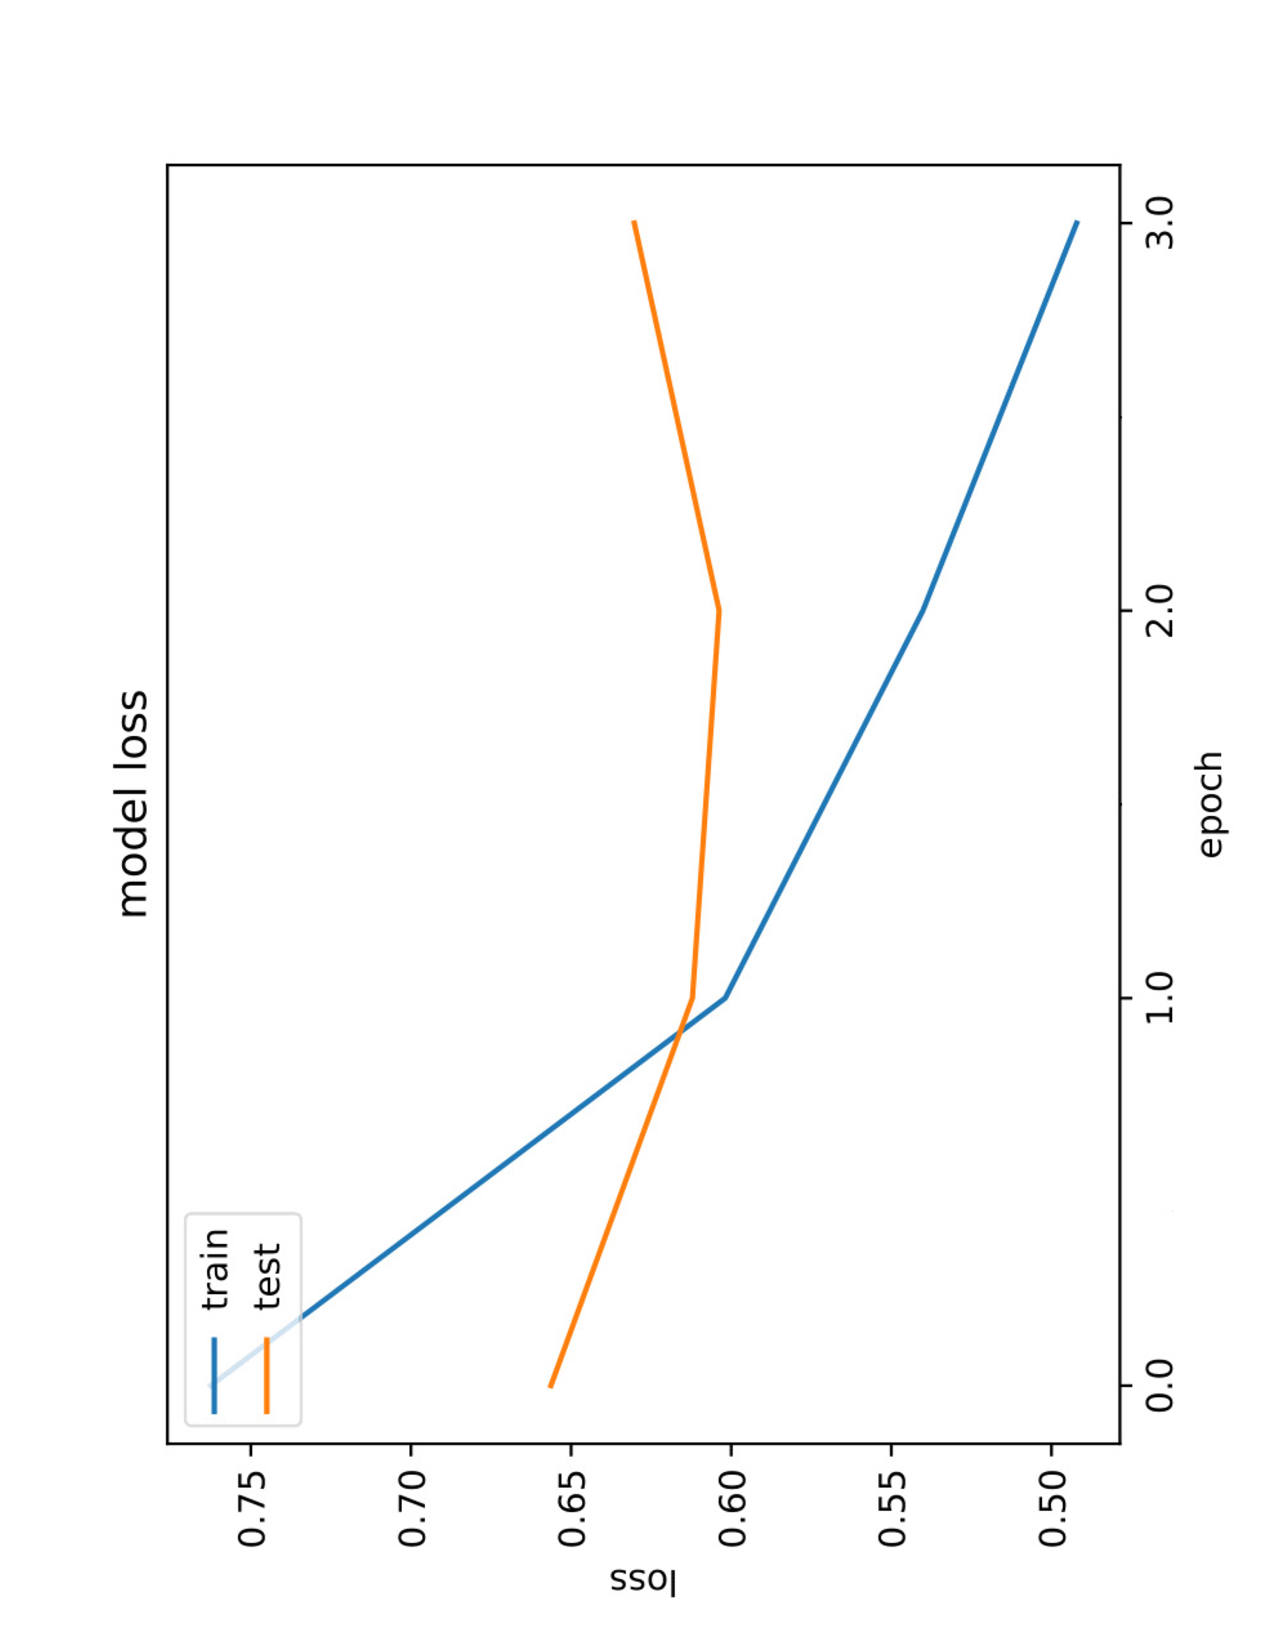
\includegraphics{gru_loss.pdf}
    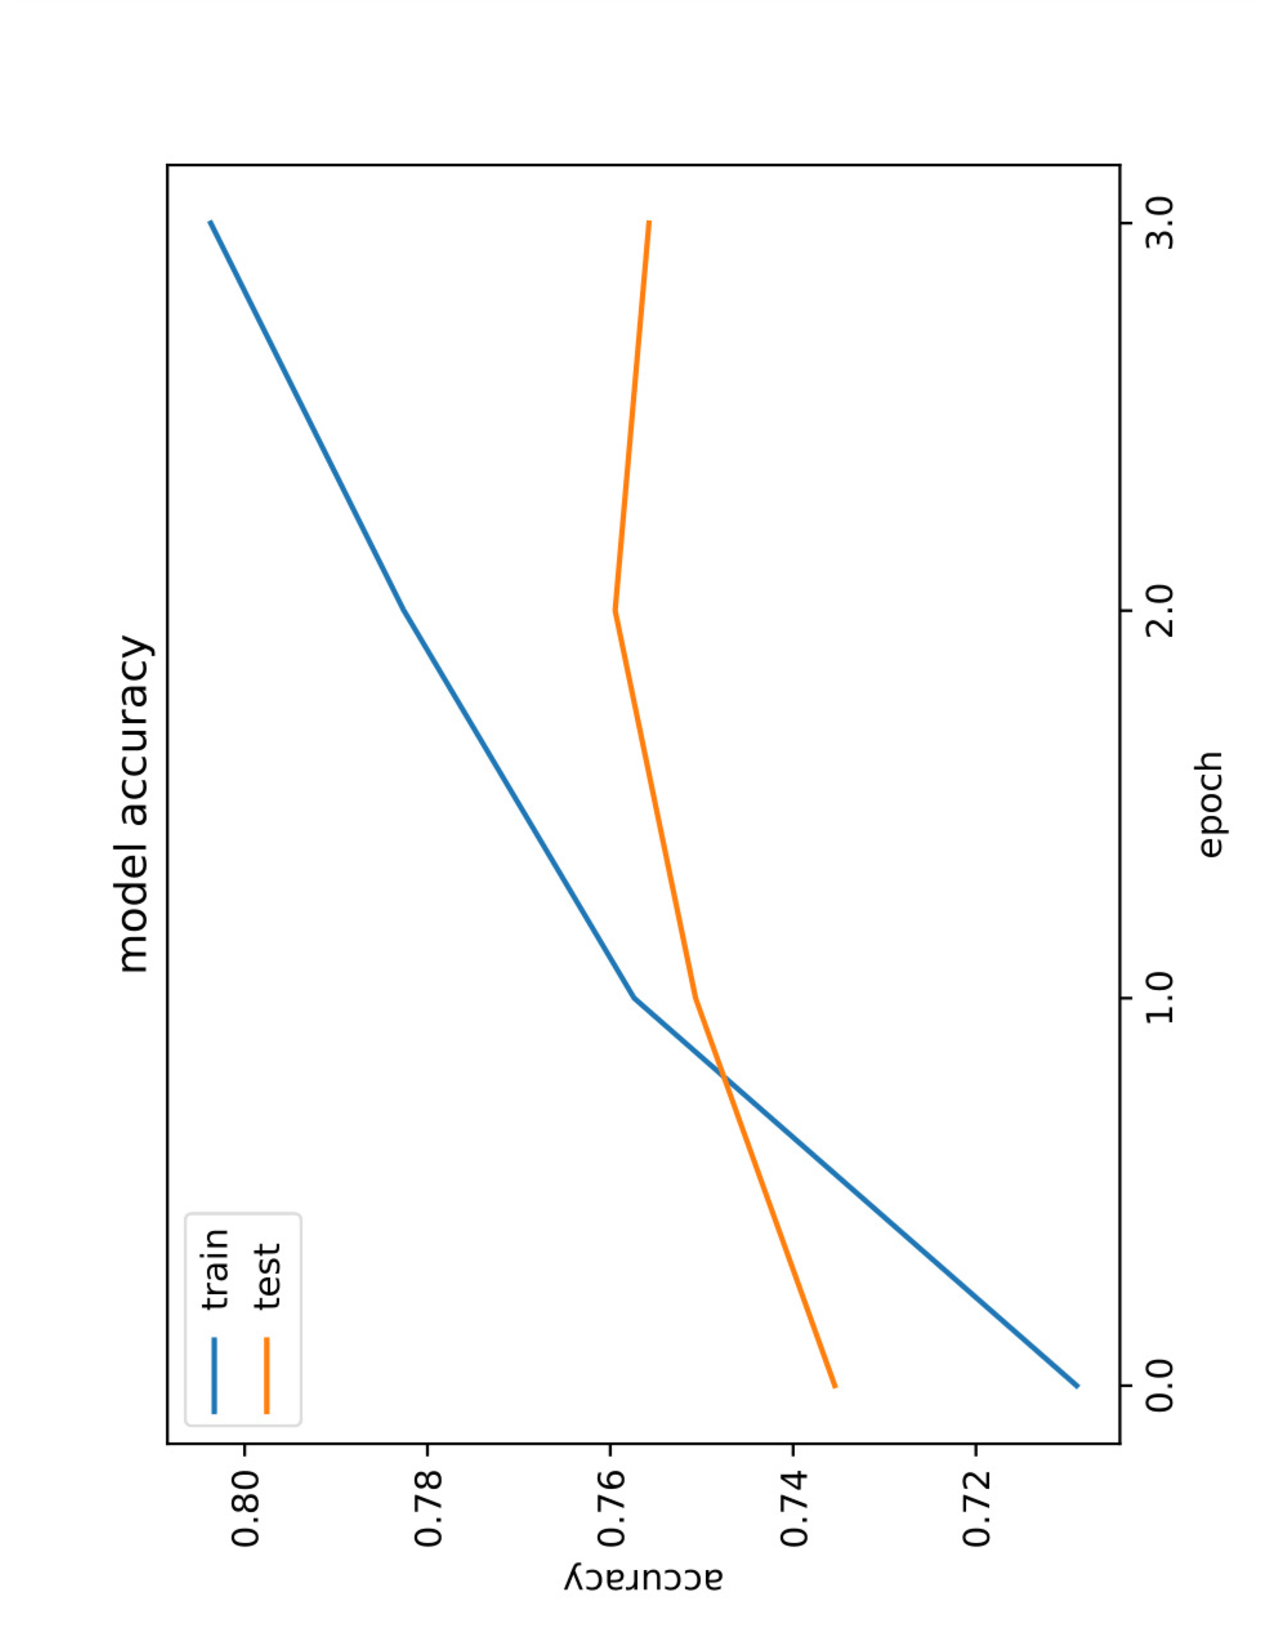
\includegraphics{gru_accuracy.pdf}
    \caption{GRU model loss and accuracy}
    \label{fig:gru}
\end{figure}
\begin{figure}[h!]
    \centering
    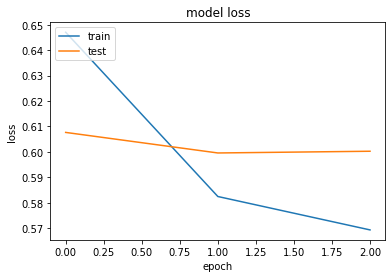
\includegraphics{trans_loss.png}
    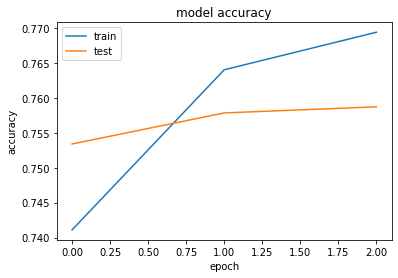
\includegraphics{trans_acc.png}
    \caption{TFBertModel model loss and accuracy}
    \label{fig:tr}
\end{figure}
\medskip
\begin{thebibliography}{12}
    
    \bibitem{imdb} 
    tf.keras.datasets.imdb.load\_data
    \\\url{https://www.tensorflow.org/api\_docs/python/tf/keras/datasets/imdb/load\_data}

    \bibitem{gru} 
    Understanding GRU Networks
    \\\url{https://towardsdatascience.com/understanding-gru-networks-2ef37df6c9be}

    \bibitem{lstm} 
    Long Short-Term Memory (LSTM): Concept
    \\\url{https://medium.com/\@kangeugine/long-short-term-memory-lstm-concept-cb3283934359\#:~:text=LSTM\%20is\%20well\%2Dsuited\%20to,and\%20other\%20sequence\%20learning\%20methods.\&text=The\%20structure\%20of\%20RNN\%20is,hidden\%20Markov\%20model.}
    
    \bibitem{Textclassification}
    Text classification with an RNN
    \\\url{https://www.tensorflow.org/tutorials/text/text\_classification\_rnn}

    \bibitem{BERT}
    Multi-Label, Multi-Class Text Classification with BERT, Transformers and Keras
    \\\url{https://towardsdatascience.com/multi-label-multi-class-text-classification-with-bert-transformer-and-keras-c6355eccb63a}

    \bibitem{BERTpros}
    BERT Explained: State of the art language model for NLP
    \\\url{https://towardsdatascience.com/bert-explained-state-of-the-art-language-model-for-nlp-f8b21a9b6270}

    \bibitem{trans}
    What is a Transformer?
    \\\url{https://medium.com/inside-machine-learning/what-is-a-transformer-d07dd1fbec04}

    \bibitem{emd}
    Deep Learning \#4: Why You Need to Start Using Embedding Layers
    \\\url{https://towardsdatascience.com/deep-learning-4-embedding-layers-f9a02d55ac12}

    \bibitem{graph}
    turicreate.recommender.create
    \\\url{https://towardsdatascience.com/deep-learning-4-embedding-layers-f9a02d55ac12}
    \\\url{https://apple.github.io/turicreate/docs/api/generated/turicreate.recommender.create.html#turicreate.recommender.create}

    \end{thebibliography}

\end{document}
